\chapter{\label{ch:protodune}The ProtoDUNE--SP Experiment} 

\minitoc

%%%%%%%%%%%%%%%%%%%%%%%%%%%%%%%%%%%%%%%%%%%%%%%%%%%%%%%%%%%%%%%%%%%%%%%%%%%%%%%%
% From COS
%
% This chapter will discuss the ProtoDUNE--SP experiment and it's role in the
% development of the proposed DUNE experiment. The LArTPC technology will be
% detailed in the general case and then the specifics of the ProtoDUNE--SP
% detector will be given. Details of the major particle fluxes in ProtoDUNE--SP
% will be outlined, along with a discussion of the simulation and reconstruction
% of each flux. Finally, as my main contribution to detector operations during
% data taking was developing for the ProtoDUNE--SP online monitoring system, this
% will be discussed in more depth. 
% 
% The work for the online monitoring subsection has been completed as part of my
% duties as an on--site expert at CERN. I expect to be able to complete the rest
% of the work by the end of December 2019 alongside the other analysis work.
%%%%%%%%%%%%%%%%%%%%%%%%%%%%%%%%%%%%%%%%%%%%%%%%%%%%%%%%%%%%%%%%%%%%%%%%%%%%%%%%

\protodune{} is one of two prototypes for the DUNE far detector modules that has
been operating at the Neutrino Platform at CERN since the summer of 2018. The
experiment collected data from a charged particle beam for approximately 3 
months before Long Shutdown 2 of the Large Hadron Collider. Since then a 
programme of cosmic ray data collection has been ongoing.

This chapter will outline the technical details of the \protodune{} experiment.
Section \ref{sec:pdsp_dune} will outline the role of \protodune{} in the context
of the DUNE experiment. This will be followed by a discussion of the main
elements of the experiment, the \protodune{} detector systems and the H4
beamline, in Sections \ref{sec:pdsp_detector} and \ref{sec:h4} respectively.
The high event rate in \protodune{} is dominated by a high flux of cosmic rays
which will be discussed in Section \ref{sec:pdsp_cosmic}. Section
\ref{sec:pdsp_sim_reco} will then discuss the simulation and reconstruction of 
\protodune{} data. Finally Section \ref{sec:pdsp_om} will cover details of the 
online monitoring system in \protodune{}; as the primary developer and expert 
on the \protodune{} online monitoring system during my time at CERN, the 
development and maintenance of this system represent a significant body of 
work over 12 months.  

\section{\protodune{} in the Context of DUNE} \label{sec:pdsp_dune}

\begin{figure}

	\centering

	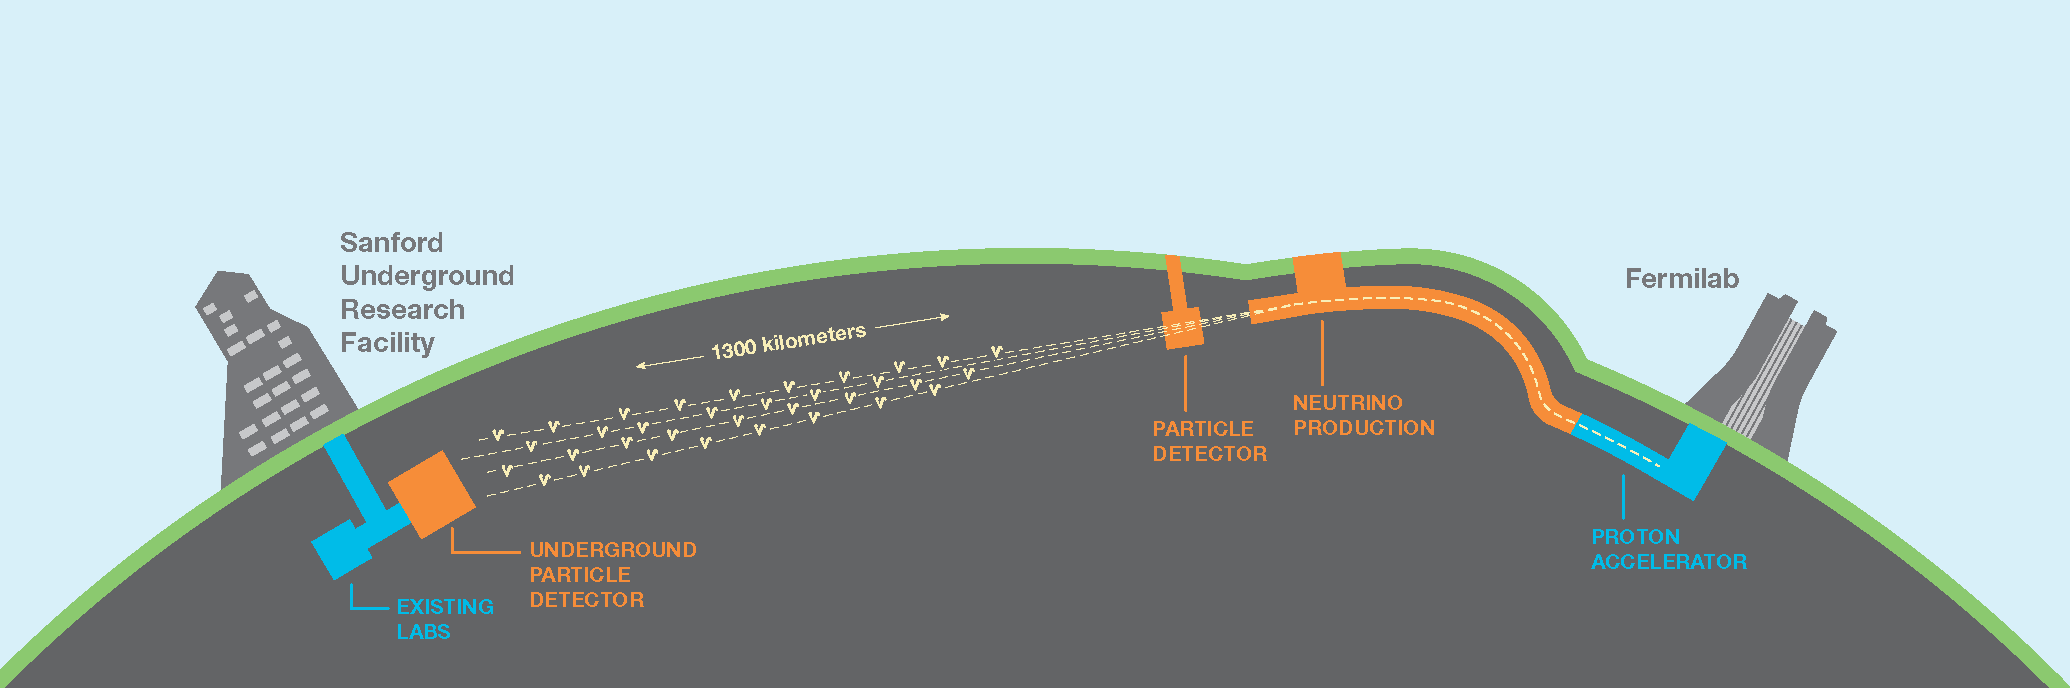
\includegraphics[width=\textwidth]{figures/dune_baseline.png}

	\caption
	[The Deep Underground Neutrino Experiment.]
	{The Deep Underground Neutrino Experiment. Figure from \cite{Abi:2020wmh}.}

	\label{fig:dune_baseline}

\end{figure}

The DUNE experiment will be a next generation neutrino physics and nucleon decay
experiment consisting of three principal components; an intense broad band 
neutrino beam and precise near detector based at the Fermilab National 
Accelerator Laboratory near Chicago, and a far detector at Sanford Underground 
Research Facility in South Dakota, approximately 1300 km away from the 
neutrino source, as demonstrated in Figure \ref{fig:dune_baseline}. The DUNE 
experiment identifies three primary scientific goals 
\cite{Abi:2020evt}:
\begin{itemize}
	\item Perform a comprehensive programme of neutrino oscillation measurements
		including measurements of \dcp{}, neutrino mass ordering, and the
		$\theta_{23}$ octant.
	\item Search for proton decay in several decay modes.
	\item Measure $\nu_e$ from a core--collapse supernova if one occurs within our
		galaxy during the lifetime of the experiment.
\end{itemize}
In addition, the experiment hopes to fulfill a significant programme of
secondary science goals:
\begin{itemize}
	\item Other accelerator based neutrino physics, such as non--standard
		interactions, sterile neutrinos, and CPT violation.
	\item Measurements of neutrino properties using atmospheric neutrinos.
	\item Dark matter searches in both the near and far detectors.
	\item A programme of neutrino interaction physics studies in the DUNE near
		detector.
\end{itemize}

To achieve these goals DUNE has opted to base the near and far detector designs
on the liquid argon time projection chamber (LArTPC) technology. The DUNE
far detector will consist of four LArTPC detectors each with 10 kt of active
liquid argon mass. This technology will have never before been used on this
scale, and therefore, there has been a significant programme of LArTPC research
and development ongoing to validate and characterise the performance of the 
technology for DUNE. 

\subsection{Liquid Argon Time Projection Chambers}
A LArTPC consists of a large volume of highly--purified liquid argon immersed in
an electric field. Charged particles traversing the liquid argon produce two
primary energy depositions, a trail of ionisation electrons along their path,
and prompt ultra--violet scintillation photons. After deposition the ionisation
electrons drift in the electric field toward the charge readout plane where they
induce electrical signals. Liquid argon is transparent to its own scintillation
light and therefore the scintillation photons can travel through the argon to be
collected in a photon detection system.The LArTPC detection principal is 
illustrated in Figure \ref{fig:lartpc}. 

\begin{figure}

	\centering

	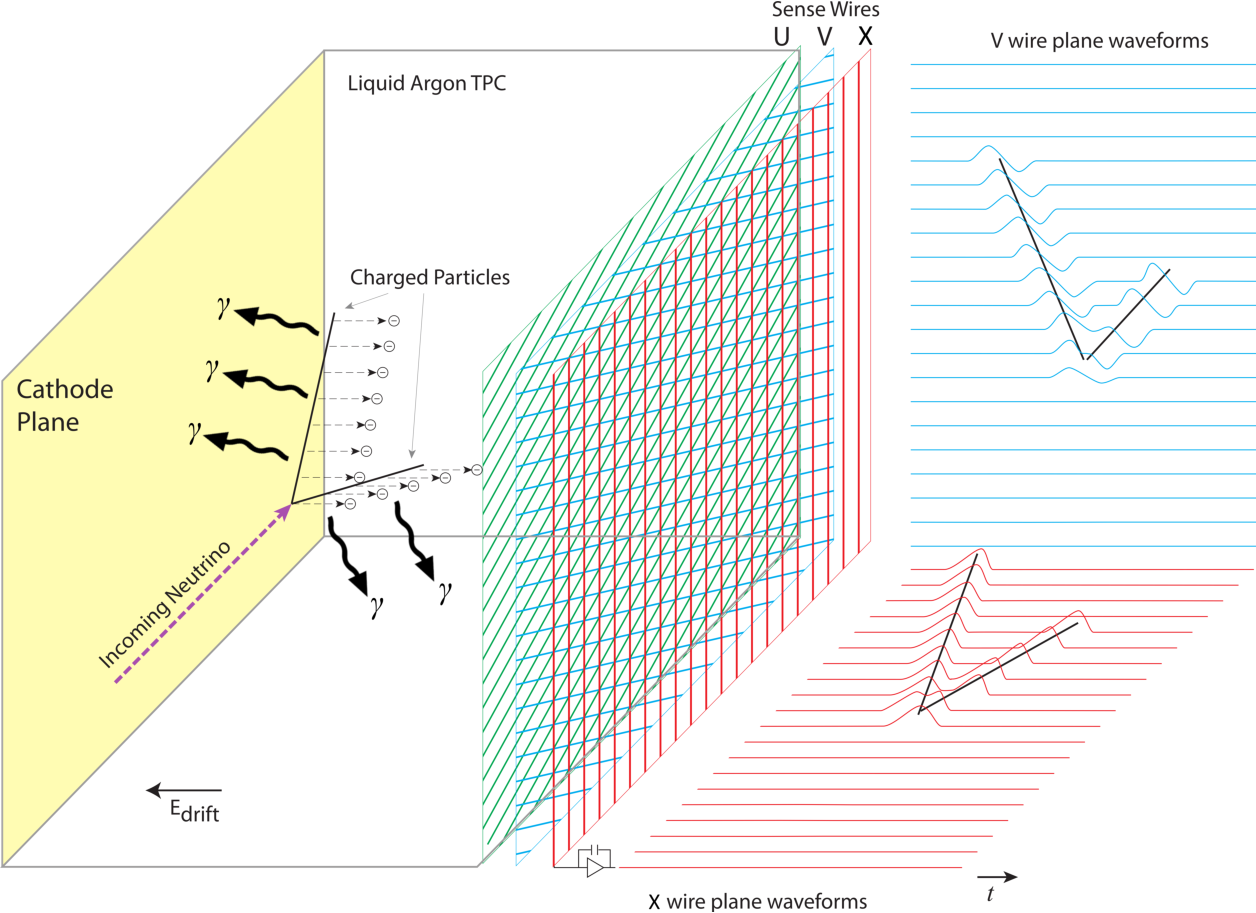
\includegraphics[width=\textwidth]{figures/LArTPC_Concept.pdf}

	\caption
	[LArTPC detection principal.]
	{LArTPC detection principal. Figure from \cite{Abi:2020loh}.}

	\label{fig:lartpc}

\end{figure}

\subsubsection*{The Role of Light in LArTPCs}

The ionisation signals in a LArTPC are slow, it takes charge milliseconds to
travel from the cathode plane to the anode plane. In contrast, scintillation 
photons only take on the order of nanoseconds to reach the closest anode 
plane. This scintillation light plays an important role in the accurate 3D 
reconstruction of interactions in the LArTPC, it provides a $t_0$. 

In a LArTPC interactions play out much quicker than the detector is able to 
record them; as such each event actually integrates over a large number of
interactions within the readout window, analogous to taking a photograph with a 
long exposure. The true time, $t_0$, of the interactions in the event cannot be 
reconstructed from the ionisation signals alone; by utilising the much faster 
scintillation signals the time of interactions can be calculated with much 
higher precision, this data can then be used to correct the position offset
caused in the ionisation signals.

\bigskip

The details of the charge readout and photon detection systems are specific to 
each detector, but broadly speaking LArTPC detectors can be split into two 
main categories: single--phase and dual--phase. In a single--phase detector the
drifting ionisation electrons remain in the liquid argon and the signals are 
typically read out on three anode wire planes. A dual--phase LArTPC contains an
additional region of gaseous argon in which a high electric field, known as the
extraction field, is applied to extract the ionisation from the liquid 
before it is amplified and collected on a pair of anode wire planes 
\cite{Abi:2020wmh}.

\bigskip

\protodune{} is one of two large scale prototypes for the DUNE far detector
modules, which focusses on the single--phase LArTPC technology. The DUNE far
detector modules feature a modular design in which each module is built up of a
number of identical components, \protodune{} was designed to prototype the
design of many of these components at a 1:1 scale, including the anode planes,
cathode plane, and photon detectors. The \protodune{} experiment has four 
primary goals, as outlined in the Technical Design Report \cite{Abi2017}:
\begin{itemize}
	\item Prototype the production and installation procedures for the
		single--phase far detector design.
	\item Validate the design from the perspective of basic detector performance;
		this can be achieved with cosmic-ray data. 
	\item Accumulate large samples of test-beam data to understand/calibrate the
		response of the detector to different particle species.
	\item Demonstrate the long-term operational stability of the detector as part
		of the risk mitigation program ahead of the construction of the first 10 kt
		far detector module.
\end{itemize}
As such, \protodune{} represents a significant milestone in the development of
the far detector for the DUNE experiment. Its successful operation, both in a 
test--beam and with cosmic rays, provides valuable data with which to understand
reconstruction and analysis of the data that will be collected by the DUNE far 
detector.

\section{The \protodune{} Detector} \label{sec:pdsp_detector}

The \protodune{} detector is located at the Neutrino Platform at CERN along the
H4 beamline. It is a single--phase LArTPC detector with a total liquid argon 
mass of 0.77 kt, making it the largest monolithic single--phase liquid argon TPC
to be built to date. The TPC comprises the following major components, which 
are illustrated in Figure \ref{fig:pdsp_tpc}:
\begin{itemize}
	\item A cathode plane constructed of modular Cathode Plane Assemblies (CPA).
	\item Two anode planes constructed of modular Anode Plane Assemblies (APA).
	\item A photon detection system (PDS) which is integrated into the APAs.
	\item A field cage (FC), beam plug, and high voltage systems (HV).
	\item Readout electronics.
\end{itemize}
The detector components are designed to be an almost exact replica of the final 
single--phase far detector modules, but the detector has an overall scaling 
factor of approximately $1:20$ in terms of total liquid argon mass 
\cite{Abi2017}.

\begin{figure}

	\centering

	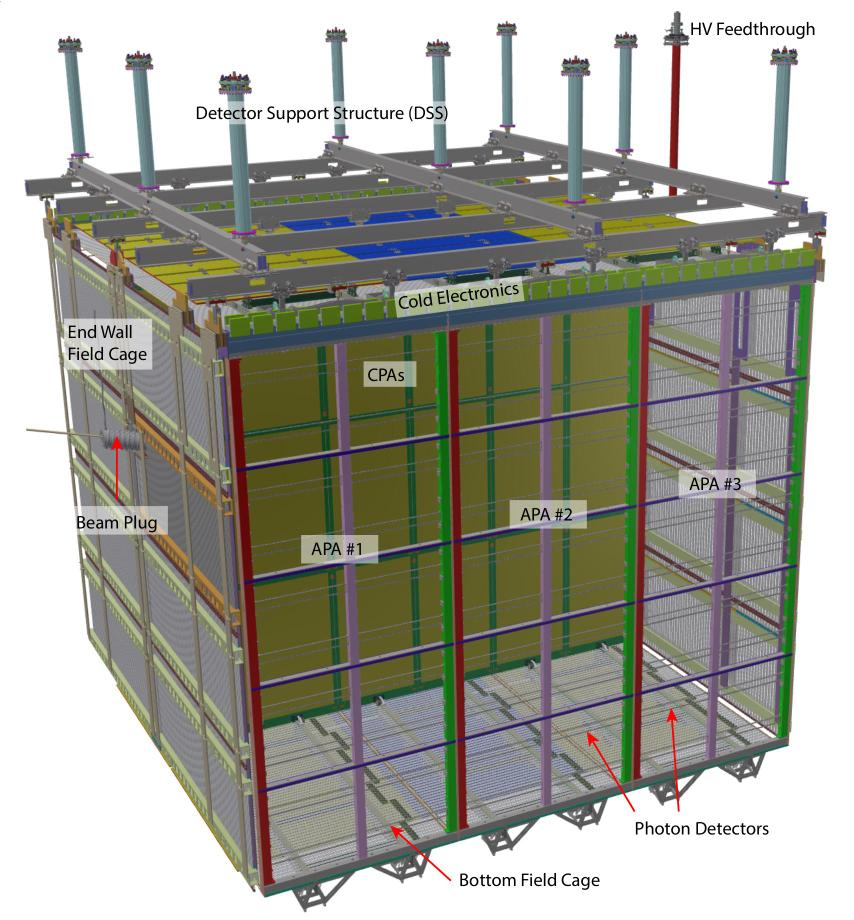
\includegraphics[width=0.9\textwidth]{figures/pdsp_tpc.jpg}

	\caption
	[The main components of the \protodune{} TPC.]
	{The main components of the \protodune{} TPC. Figure from \cite{Abi2017}.}

	\label{fig:pdsp_tpc}

\end{figure}

\subsection{The Liquid Argon TPC}

The \protodune{} TPC has an active volume of 6 m (height) $\times$ 7.2 m (width,
drift direction) $\times$ 7 m (length, approximate beam direction). The cathode 
plane at the center of the active width is flanked by two anode planes which 
define two 3.6 m drift volumes. The field cage around these two drift volumes
helps to ensure a uniform electric field within the drift region.

Each anode plane is modularly constructed from three APAs which have dimensions
6 m (height) $\times$ 2.3 m (width). The APA frame holds three sets of parallel
wires on the inward and outward facing sides, these are oriented at different 
angles to enable 3D reconstruction. The first two sets of wires are induction
wires, these are electrically connected and biased such that they are
electrically transparent to the drifting ionisation; ionisation passing the
induction wires causes an induced bi--polar signal. The third set of wires are 
known as collection wires, they are not electrically connected; when drifting 
ionisation approaches the collection wires it is absorbed producing a 
uni--polar signal. In \protodune{} each set of induction wires contains 800
wires at a 4.67 mm pitch, and each set of collection wires contains 480 wires at
a 4.79 mm pitch. 

The wire planes from each APA are read out by electronics mounted on the APA 
frame; these electronics are submerged in the liquid argon and therefore 
referred to as cold electronics (CE). A total of 2560 electronics channels are 
used to read out the data from each APA. The CE amplify, shape, and digitise the
signals from the wires before transmitting them outside the TPC to the Warm
Interface Boards (WIB). The WIBs collate the data from the CE boards along with
timing information from the timing system and pass the data onto the 
Data Acquisition System (DAQ).

The cathode plane in \protodune{} consists of an array of 18 CPA modules, 2 m 
(height) $\times$ 1.2 m (width). The cathode plane is held at -180 kV to 
provide a 500 $\mbox{Vcm}^{-1}}$ drift field in each of the drift volumes. The 
field cage surrounding the drift regions ensures that the electric field is 
uniform across the detector volume. \mccorrect{How does it do this? Equally
spaced resistors I think.}

One area in which the design of \protodune{} differs from the far detector is
the inclusion of the beam plug. This is necessary to minimize interactions
between the charged particle test--beam and the cryostat before the beam enters 
the active region of the detector. A cylindrical beam plug, containing 
nitrogen gas, penetrates from the cryostat wall into the field cage at 
location of the incoming test--beam. 

\subsection{The Photon Detection System}

The PDS in \protodune{} is integrated into the APAs. Ten photon detector modules
are embedded in each APA frame between the layers of wires on each APA 
face, as shown in Figure \ref{fig:pdsp_tpc}. Three types of photon detector
module were tested in \protodune{}, two very similar module designs based on
wavelength coupling silicon photomultipliers to wavelength shifting bars, and a
third novel design know as the ARAPUCA light trap. The operating principles of
the two designs are illustrated in Figure \ref{fig:pdsp_pd}.

\begin{figure}

	\centering

	\begin{subfigure}[b]{0.28\textwidth}
		\centering
		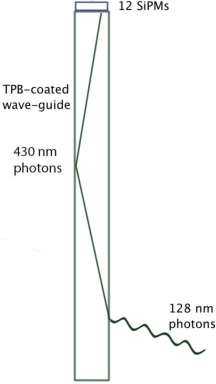
\includegraphics[height=0.3\textheight]{figures/pdsp_pd.pdf}
		\caption{Waveguide.}
		\label{fig:pd_bars}
	\end{subfigure}
	\hfill
	\begin{subfigure}[b]{0.67\textwidth}
		\centering
		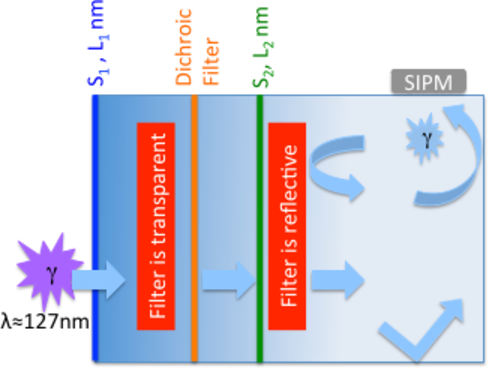
\includegraphics[height=0.3\textheight]{figures/pdsp_arapuca.pdf}
		\caption{ARAPUCA.}
		\label{fig:arapuca}
	\end{subfigure}

	\caption
	[The operating principal of the photon detector modules in \protodune{}.]
	{The operating principal of the photon detector modules in \protodune{}.
	Figure \subref{fig:pd_bars} from \cite{Abi2017}. Figure \subref{fig:arapuca} 
	from \cite{Machado:2016jqe}}

	\label{fig:pdsp_pd}

\end{figure}

The majority of the photon detector modules in \protodune{} consist of 
wavelength shifting bars coupled to silicon photomultipliers (SiPM). 
Tetraphenyl-butadiene (TPB) is used to shift the wavelength of the light 
ultra--violet to blue before the light is transmitted down the waveguide to 
the SiPMs. The main difference between the two nominal designs is in the 
wavelength of transmission within the waveguide; in one case the wavelength is 
transmitted at the blue wavelength produced by the TPB, in the other case the 
blue light from the TPB is first absorbed in the waveguide which then produces 
green light which is transmitted down the waveguide.

A small number of the photon detector modules in \protodune{} feature a novel 
design known as an ARAPUCA light trap. In this design the photons are trapped 
in a small box through a sequence of wavelength shifting and optical 
filtering, significantly increasing the photon detection efficiency 
\cite{Segreto:2018jdx}. An ARAPUCA light trap consists of a 5 cm $\times$ 5 cm 
$\times$ 1 cm box which is coated with a highly reflective surface, on one 
side of the box is the filtering window, and on the other a SiPM. Incoming 
ultra--violet photons are shifted to the blue spectrum before passing through 
a dichroic filter which has a tunable wavelength cut--off at which it 
transitions from being transparent to reflective. After passing through the 
filter the photons are shifted again, this time from blue to green, such that 
when they get back to the filter it is reflective. As such green photons can 
be trapped within the ARAPUCA until they come into contact with the SiPM, 
providing increased photon detection efficiency. Each ARAPUCA photon detector 
module in \protodune{} features TODO of these traps arranged in a line across 
the width of an APA.

Unlike with the TPC electronics, there are no front--end electronics in the LAr
volume for the PDS, the unamplified analogue signals are transmitted out of the
cryostat before processing and digitisation. Each photon detector module has 
12 SiPMs which are read out in threes such that each module corresponds to 4 
readout channels. The 40 readout channels from each APA are processes by four 
so called SiPM Signal Processors (SSP), which handle 10 channels each and are 
mounted on the top of the cryostat. After processing in the SSPs the PDS data is
passed onto the DAQ along with the TPC data.

\section{The H4 beamline} \label{sec:h4}

The \protodune{} experiment is located at the end of the H4 beamline at CERN,
the location of the beamline with respect to the detector is illustrated in
Figure \ref{fig:pdsp_CRT}.  The beam can be configured to provide hadron, 
muon, and electron beams with energies in the range 1--7 GeV into the 
detector. 

The H4 beamline as a tertiary beamline which is produced when a secondary beam
from the T2 primary target interacts with a secondary target. Particles from the
secondary beam are selected based on momentum and charge before travelling down
the H4 beamline to \protodune{}. A schematic of the beamline instrumentation
(BI) and magnets in the H4 beamline is given in Figure \ref{fig:h4_schem}. 

\begin{figure}

	\centering

	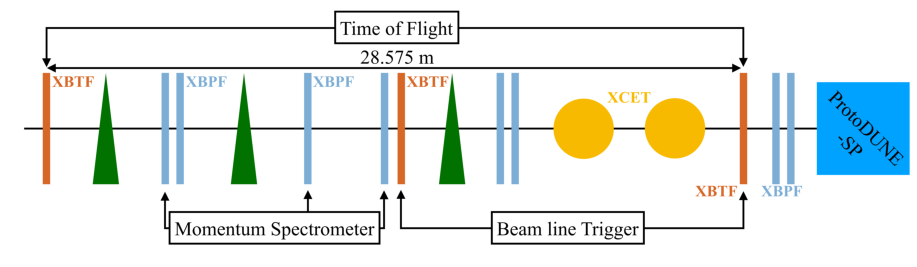
\includegraphics[width=\textwidth]{figures/h4_schem.pdf}

	\caption
	[Schematic of the H4 beamline magnets and instrumentation.]
	{Schematic of the H4 beamline magnets and instrumentation. Figure from
	\cite{protoduneperf}.}

	\label{fig:h4_schem}

\end{figure}

By combining momentum measurements from the profile monitors with time of flight
(TOF) and Cerenkov measurements the beam momentum and composition can be 
measured. The predicted and measured distribution of TOF vs momentum for data 
from a number of runs at different momenta is shown in Figure \ref{fig:h4_tof}.
This information is used to trigger the detector during beam running, and is
sent to the central trigger board for distribution to the detector components.

\begin{figure}

	\centering

	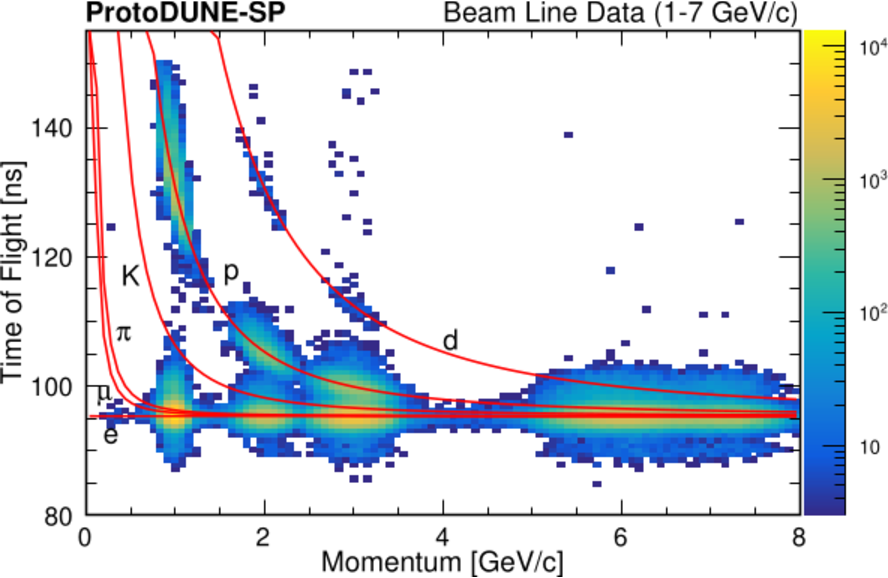
\includegraphics[width=\textwidth]{figures/h4_tof.pdf}

	\caption
	[Time of flight vs momentum distributions from the H4 beamline
	instrumentation.]
	{Time of flight vs momentum distributions from the H4 beamline
	instrumentation. Figure from \cite{protoduneperf}}

	\label{fig:h4_tof}

\end{figure}

\section{The Cosmic Ray Tagger} \label{sec:pdsp_cosmic}

As a surface level detector with no overburden \protodune{} measures a
significant rate, on the order of 20 kHz, of cosmic ray muons, corresponding 
to an average of 60 muons per 3 ms readout window. These muons provide a 
useful source of calibration data in to form of long tracks and stopping muons. 
The Cosmic Ray Tagger (CRT) in \protodune{} was installed on the upstream and
downstream faces of the TPC to trigger the detector for cosmic--ray muons which
travel parallel to the anode plane. In addition the CRT provides an additional
source of $t_0$ tagged tracks for calibration.

The CRT consists of four parts, two upstream assemblies and two downstream
assemblies, the locations of the CRT assemblies is illustrated in Figure
\ref{fig:pdsp_CRT}. Each CRT assembly is constructed from overlapping 
scintillation counters which cover an area 6.8 m high and 3.65 m wide. 
Scintillation strips of length 365 cm and width 5 cm are placed in 
perpendicular arrays to give two--dimensional reconstruction within each CRT 
assembly. By combining data from upstream and downstream CRT assemblies with a 
time coincidence requirement the trajectories of tracks can be reconstructed.

\begin{figure}

	\centering

	\begin{subfigure}[b]{\textwidth}
		\centering
		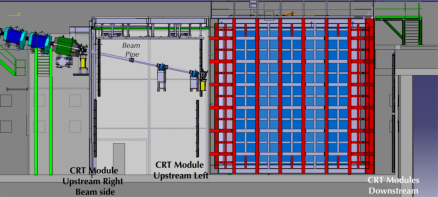
\includegraphics[width=0.6\textwidth]{figures/crt_side.pdf}
		\label{fig:crt_side}
		\caption{Side view.}
	\end{subfigure}

	\vspace{3mm}

	\begin{subfigure}[b]{\textwidth}
		\centering
		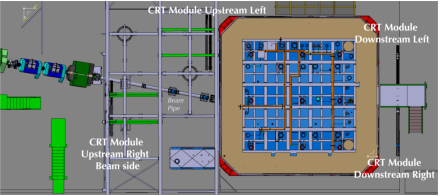
\includegraphics[width=0.6\textwidth]{figures/crt_top.pdf}
		\label{fig:crt_top}
		\caption{Top view.}
	\end{subfigure}

	\caption
	[Location of the H4 beamline and cosmic ray taggers in relation to the
	\protodune{} detector.]
	{Location of the H4 beamline and cosmic ray taggers in relation to the
	\protodune{} detector. Figures from \cite{protoduneperf}.}

	\label{fig:pdsp_CRT}

\end{figure}

\section{The Data Acquisition System}

Data from the TPC, PDS, and CRT in \protodune{} are collated by the Data 
Acquisition system (DAQ). The DAQ distributes triggers, compresses and packages 
the data into events, monitors the data quality, and stores the data ready for 
future analysis. An overview of the \protodune{} DAQ system is seen in Figure 
\ref{fig:pdsp_daq}; there are four primary data flows in the system: TPC, PDS,
CRT, and BI. Timing and triggering signals are distributed to the detector 
components by the timing board which maintains a 50 MHz clock and receives 
$\sim 40 \mbox{Hz}$ of triggers from the Central Trigger Board (CTB) based on 
data from the BI and CRT \cite{Abi2017}.

\begin{figure}

	\centering

	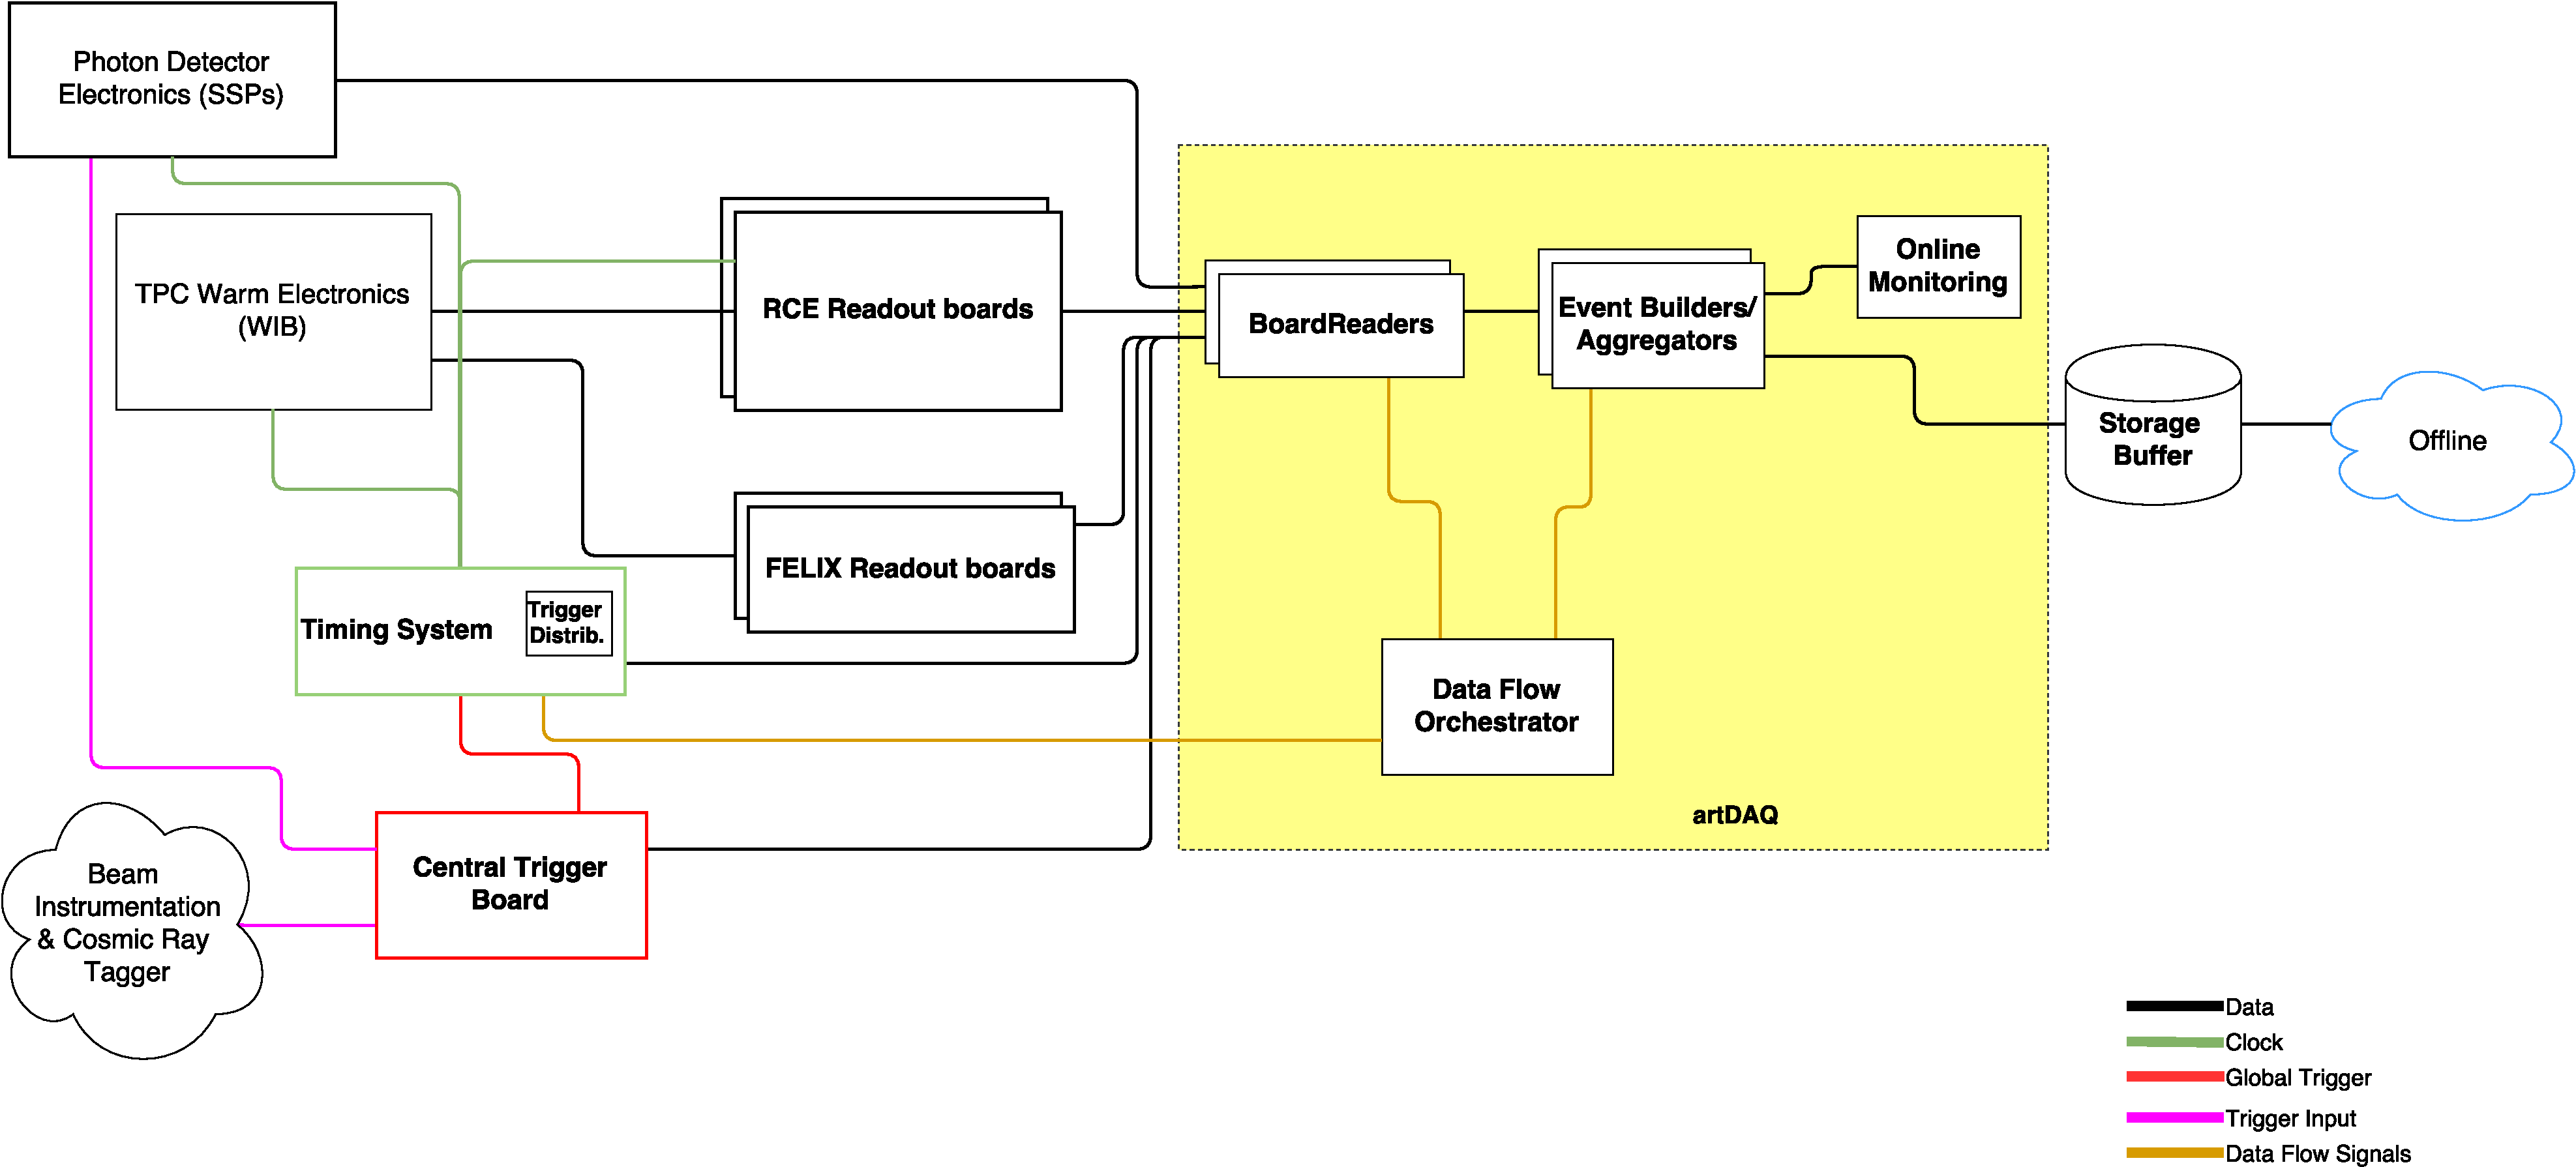
\includegraphics[width=\textwidth]{figures/pdsp_daq.pdf}

	\caption
	[Outline of the data acquisition system in \protodune{}.]
	{Outline of the data acquisition system in \protodune{}. Figure from
	\cite{Abi2017}.}

	\label{fig:pdsp_daq}

\end{figure}

The \protodune{} TPC contains a total of 15,360 wires spread across the six
APAs, the wires are digitized at a rate of 2 MHz resulting in an overall data
flow of around 480 $\mbox{Gb s}^{-1}$ from the TPC electronics. An event in
\protudune{} corresponds to a continuous readout of the detector for 3 ms,
resulting in 6000 samples from each wire; data is buffered such that the readout
window can be opened 250 $\mu$s before the trigger time. Data from the TPC is
received by two systems, a system based on Reconfigurable Computing Elements
(RCE) \cite{7431254} handles the data from five APAs while data from the sixth 
is received by a system based on Front--End Link Exchange (FELIX) cards which 
have been developed by the ATLAS collaboration \cite{Anderson_2016}.

The software layer of the \protodune{} DAQ is based on Fermilab's artdaq 
\cite{6495515}. This component is primarily responsible for acquiring the data,
packaging it, and storing it locally. Triggered events are queued and 
distributed to the board readers and event builders by the Data Flow 
Orchestrator. There are multiple board readers which are each responsible for 
processing the data from specific hardware components, details vary between 
specific board readers but generally these processes are responsible for 
formatting the data from each component ready for aggregation. Data from the
various detector components are aggregated by the event builders, which are
responsible for assembling the completed events. After compression events have
an average size of 60 MB. Artdaq is also responsible for the real--time 
monitoring of data quality via the online monitoring system, this system will be
discussed in Section \ref{sec:pdsp_om}.

\section{Simulation and Reconstruction} \label{sec:pdsp_sim_reco}
TODO.

\section{ProtoDUNE--SP Online Monitoring System} \label{sec:pdsp_om}
